\chapter{Activiti BPM}\label{chp:activiti}

\section{Introdução}\label{sec:activiti-introducao}
Criado em 2010 por ex-integrantes do projeto jBPM, o Activiti BPM é um projeto de código aberto sob a licença Apache V2, que provê um motor BPM leve e completo sob a especificação BPMN 2.0. O Activiti é desenvolvido sob a linguagem de programação Java e é facilmente integrável com aplicações existentes por sua leveza e API amigável.

Neste capítulo vamos apresentar como o Activiti BPM pode ser utilizado na automatização de processos de negócio. Vamos apresentar ainda, a capacidade de modelagem de processos através da notação BPMN utilizada pelo Activiti. Por último vamos abordar as vantagens e limitações desta ferramenta frente às demais opções do mercado.

\section{BPMN}\label{sec:activiti-bpmn}
A BPMN (Business Process Management Notation) foi criada para representar processos de negócio em forma de diagrama, através de uma notação padronizada e de fácil entendimento por diferentes profissionais, sejam desenvolvedores, analistas de negócio ou gestores. Foi criada inicialmente pelo BPMI (Business Process Management Initiative) em 2004, mas atualmente é mantida e atualizada pela OMG (Object Management Group). Sua versão mais atual é a BPMN 2.0, publicada em 2011.

A notação foi concebida sob a perspectiva de cobrir a falta de entendimento entre diferentes departamentos e organizações a cerca de um determinado processo ou conjunto de processos, algo muito frequente no ambiente corporativo. Além disso, através de sua notação padronizada em XML (Extensible Markup Language), diferentes ferramentas podem fazer o uso de sua auto-descrição para orquestração de processos de negócio, sejam eles automatizáveis ou não.

A notação define quatro grupos distintos de objetos para permitir a diagramação de um fluxo de negócio. Os objetos são classificados em artefatos, agrupadores, conectores e objetos de fluxo. São utilizadas figuras geométricas, como retângulos e círculos, além de linhas pontilhadas e tracejadas, entre outros elementos para representar cada um dos objetos que constituem a notação.

1) http://searchcio.techtarget.com/definition/Business-Process-Modeling-Notation

2) http://blog.iprocess.com.br/2012/11/um-guia-para-iniciar-estudos-em-bpmn-i-atividades-e-sequencia

3) https://www.fluig.com/blog/entendendo-melhor-o-bpmn/

\begin{figure}
  \centering
  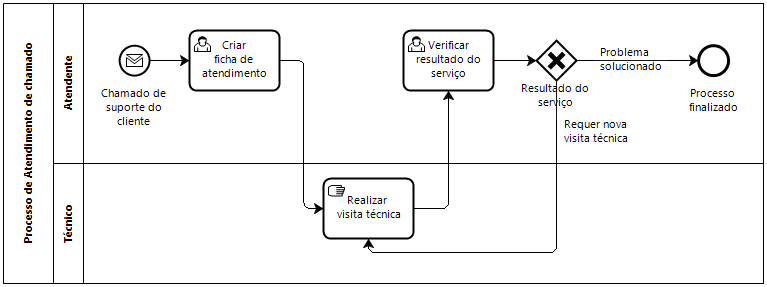
\includegraphics[width=1.0\textwidth]{imagens/bpmn_example.png}
  \caption{Exemplo de processo representado em BPMN}
  \label{fig:exemplo_bpmn}
\end{figure}

\section{Gestão de processos com o Activiti BPM}\label{sec:activiti-gestao_processos}

O motor do Activiti BPM é disponibilizado através de um simples arquivo JAR, modelo de arquivo padrão para bibliotecas da linguaguem Java. Sendo assim, o motor BPM pode ser facilmente utilizado em diferentes projetos Java através da inclusão dessa biblioteca como dependência e pela utilização de sua API.
\section{Como automatizar um processo?}\label{sec:activiti-automatizar_processo}

\section{Vantagens e Limitações}\label{sec:activiti-vantages_limitacoes}


